\section{Architecture}

\vspace{1em}
\begin{minipage}{\linewidth}
    \centering
    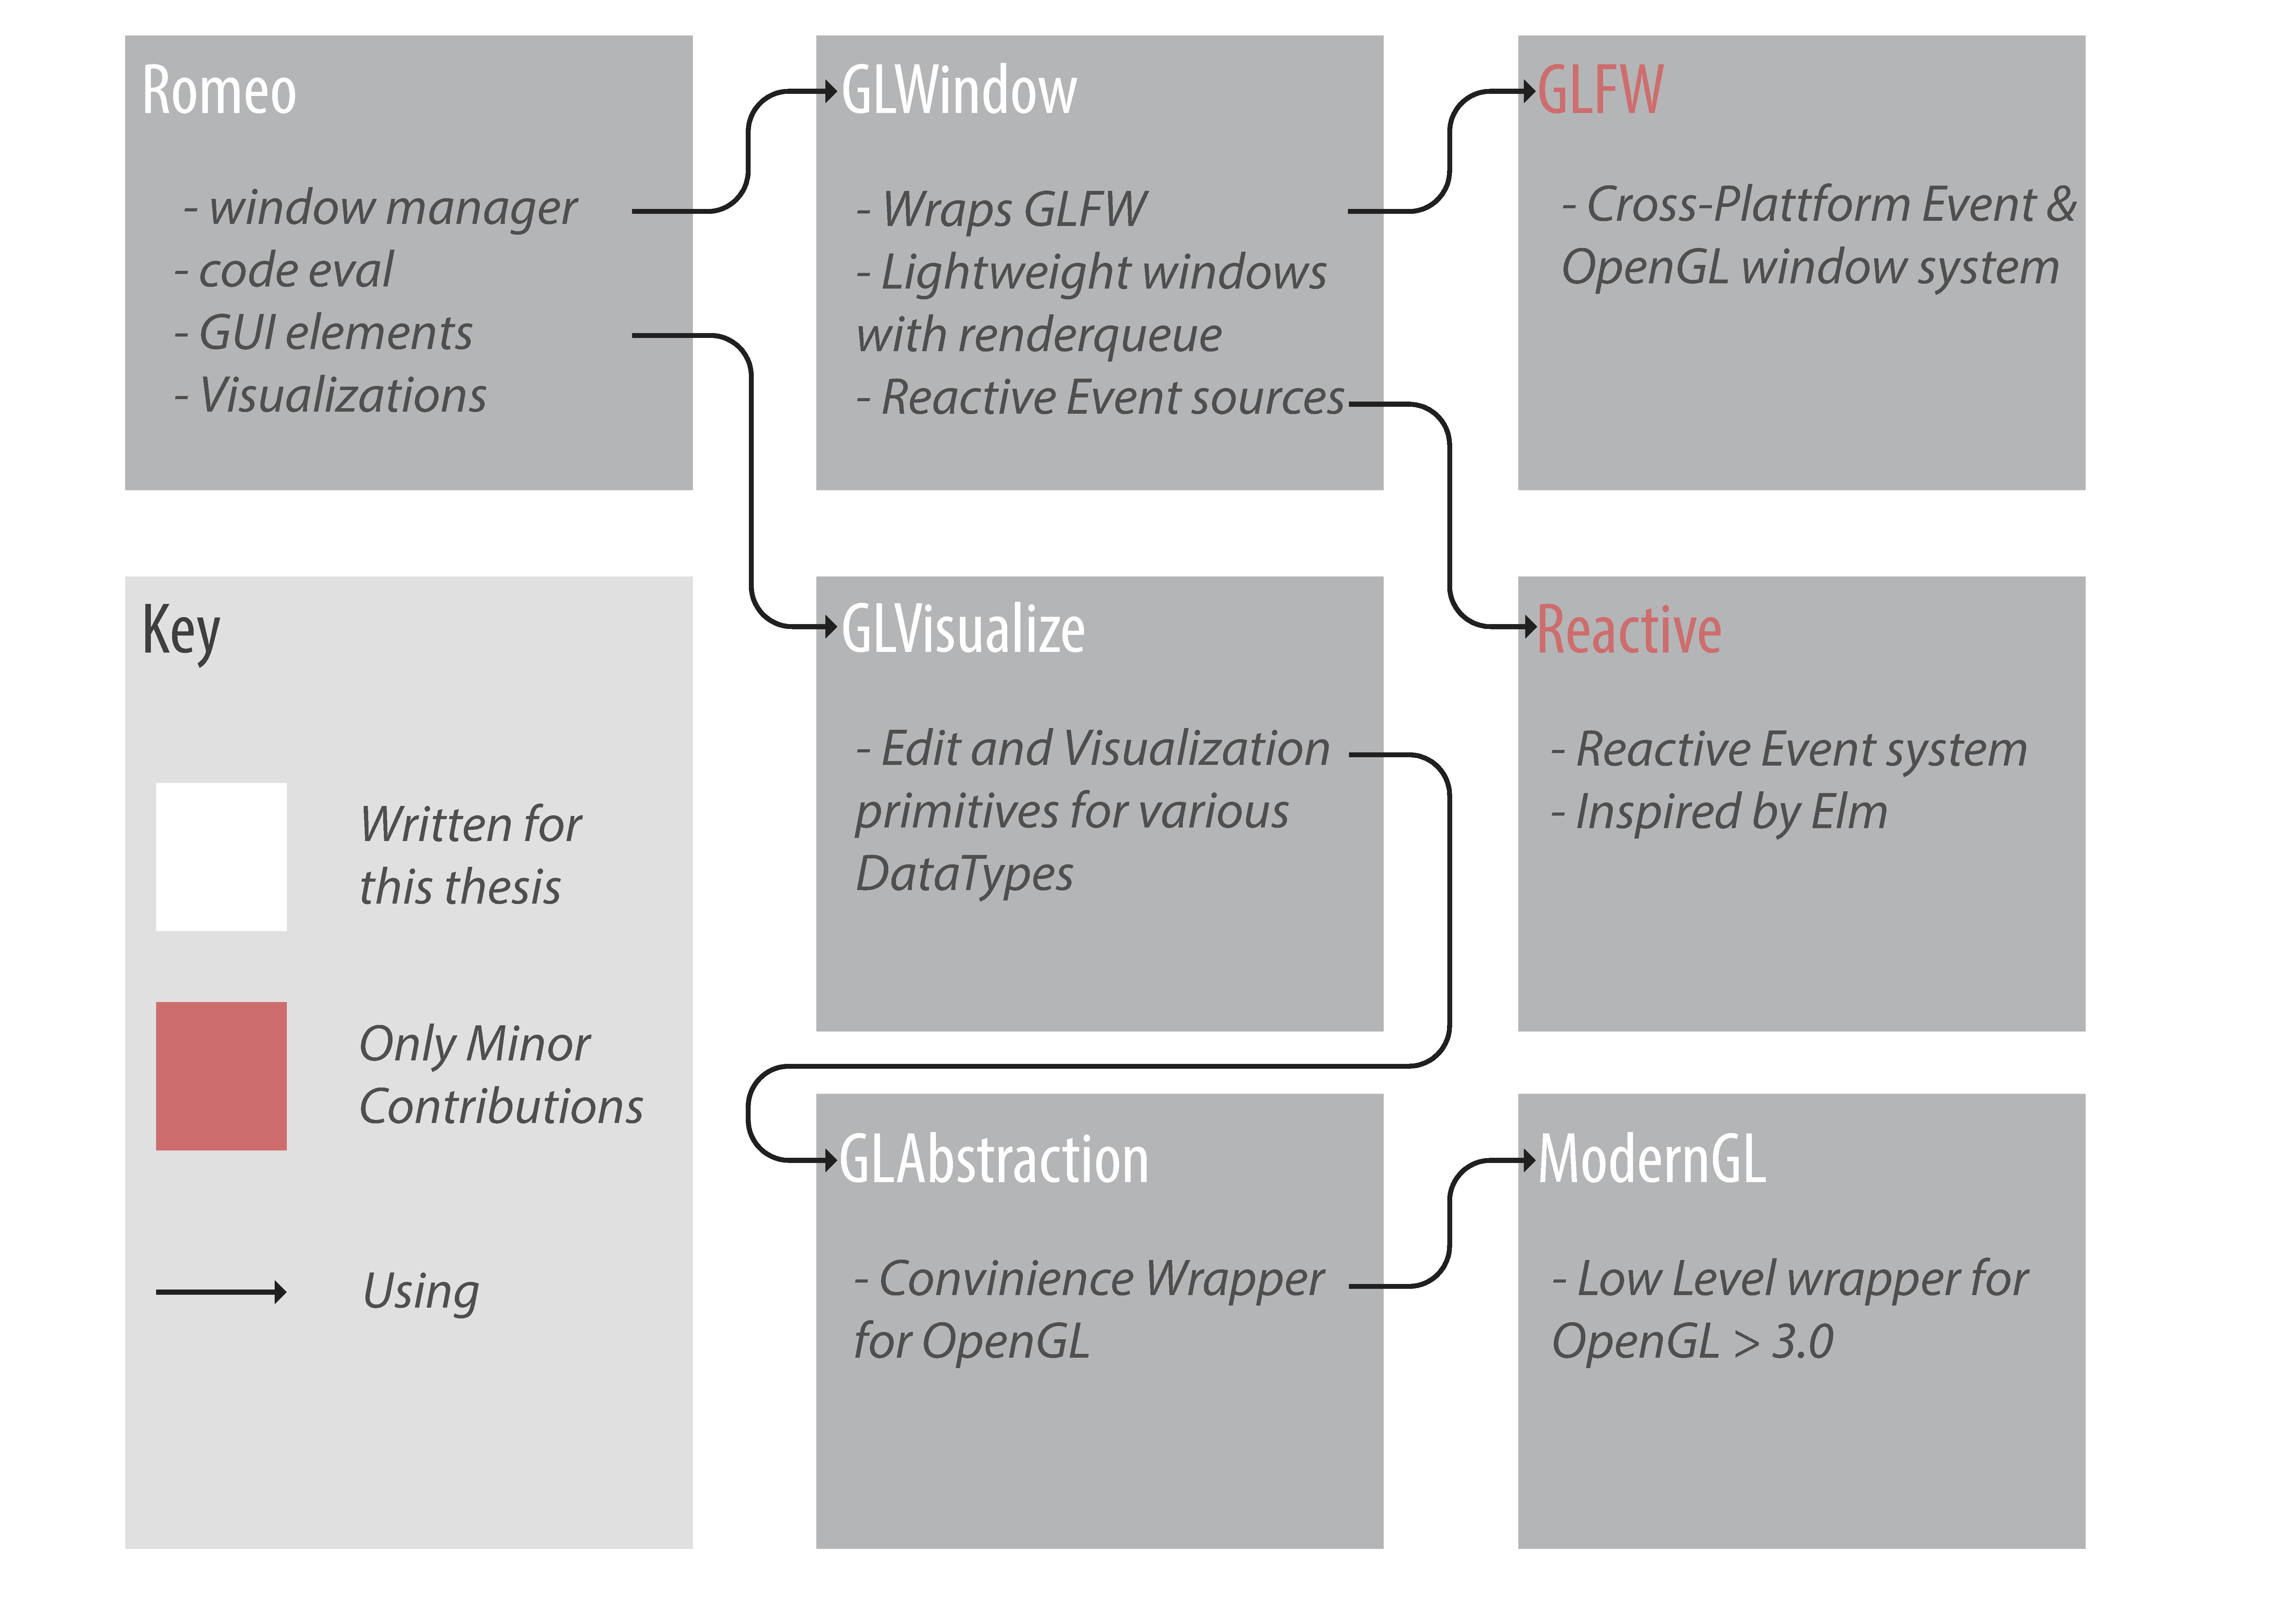
\includegraphics[width=0.9\linewidth]{graphics/architecture.pdf}
    \captionof{figure}[Architecture]{Main modules used in Romeo and their relation (simplified)}
    \label{fig:architecture} 
\end{minipage}


This chapter is about the architecture of Romeo.
Romeo itself just defines the high-level functionality of the editor.
This includes window layout and connecting all the different event sources to create the wanted behavior.
To do this, Romeo relies on a multitude of packages, which step for step abstract away the underlying low-level code that is used to do the window creation and rendering.
GLVisualize is the main package offering the rendering functionality and the editor widgets like text fields and sliders.
For rendering GLVisualize relies on GLAbstraction, which defines a high-level interface to OpenGL.
OpenGL function loading is done by ModernGL, which keeps all the function and Enums definitions from OpenGL with version higher than 3.0.
The event management is handled by Reactive, which is a reactive event system written in Julia.

\subsection{Reactive}

Reactive is an reactive event system, designed for event driven programming.
Its building blocks are signals, which are values that change over time.
These signals can be transformed via arbitrary functions which creates a new signal. 
\begin{lstlisting}
a = Input(40) # an integer signal.
b = Input(2) # an integer signal.
c = lift(+, a,b) # creates a new signal with the value 42
lift(println, c) 
push!(a, 20) # updates a, resulting in c being 22
#output -> 22
push!(a, 20) # updates a, resulting in c being 22
#output -> 22
\end{lstlisting}


\subsection{ModernGL}
OpenGL is implemented by the video card vendor and is shipped via the video driver, which comes in the form of a C-Library.
The challenge is, to load the function pointer system and vendor independently. Also one further complication is, that depending on the platform, function pointer are only available after an OpenGL context was created and may only be valid for this context. \cite{wgl}
This problem is solved, by initializing a function pointer cache with null and as soon as the function is called the first time the real pointer gets loaded. This is suboptimal, as the pointer cannot be inlined and has to be checked for null.
In the newest version of Julia, this can be implemented even more efficiently with staged functions. Staged functions can be thought of as a runtime macro.
At the first call of the function code can be generated, which then will get compiled in time and replaces the function definition. 
This makes the an OpenGL function call nearly twice as fast.
Like this, even C can be outperformed in terms of speed, as C doesn't have just in time compilation capabilities, so the function pointers can not be inlined like this. [benchmark pending]


\subsection{GLAbstraction}


\subsection{GLWindow}
GLWindow is a lightweight wrapper around GLFW. GLFW is a C-Library, that offers cross-platform OpenGL window and context creation and event handling.
GLWindows is the abstraction layer, that builds upon a Julia wrapper of GLFW.
It mainly offers a screen type, which contains signals for all the different GLFW events (Mouse, Keyboard, etc...). 
It also offers a hierarchical structure for nesting screens in each other. 
All the screen areas are signals, which resize the screen area when they change. Like this, you can dynamically have the screen sizes depend on each other and react to resizing the window.



\subsection{GLVisualize}
GLVisualize implements the main functionality of this library.
It offers rendering of different primitives. GLVisiualize is designed with two intentions in mind: supplying a very simple interface consisting of just two functions and transport the data with as little conversions and copies to the GPU.
This allows to manipulate the data directly on the GPU, which is the fastest way to update dynamic data.
The interface to create visualizations is very simple and only consists of two functions:
\begin{lstlisting}
visualization 		  = visualize(data::T, style=Style{:default}; parameters...)
visualization, signal = edit(     data::T, style=Style{:default}; parameters...)
\end{lstlisting}

With this, the following data can be visualized:
\begin{itemize}
	\item Text (Vector of Glyphs)
	\item Height fields with different primitives (Matrix of height values)
	\item 3D bar plots (Matrix of height values)
	\item Images (Matrix of color values)
	\item Videos (Vector of Images)
	\item Volumes (3D Array of intensities)
	\item Particles (Vector of Points)
	\item Vector Fields (3D array of directional Vectors)
	\item Colors (Single Color values)
\end{itemize}
These can be integrated into the same scene. For all of these, it is possible to change their values interactively.
The edit function is making it easier to edit the values of the data.
It calls the visualize function to render the data type and then registers appropriate events to update the data.
Take a look at the text edit function. 
It first uploads the text to video memory and sets up the functionality to visualize it, and than updates the text data on the GPU according to the cursor position and keyboard input.

Up to now, there is only an edit function available for text fields, colors, numbers, vectors and matrices.




\subsubsection{Romeo}
